%; whizzy chapter
% -initex iniptex -latex platex -format platex -bibtex jbibtex -fmt fmt
% 以上 whizzytex を使用する場合の設定。

%     Tokyo Debian Meeting resources
%     Copyright (C) 2007 Junichi Uekawa

%     This program is free software; you can redistribute it and/or modify
%     it under the terms of the GNU General Public License as published by
%     the Free Software Foundation; either version 2 of the License, or
%     (at your option) any later version.

%     This program is distributed in the hope that it will be useful,
%     but WITHOUT ANY WARRANTY; without even the implied warranty of
%     MERCHANTABILITY or FITNESS FOR A PARTICULAR PURPOSE.  See the
%     GNU General Public License for more details.

%     You should have received a copy of the GNU General Public License
%     along with this program; if not, write to the Free Software
%     Foundation, Inc., 51 Franklin St, Fifth Floor, Boston, MA  02110-1301 USA

%  preview (shell-command (concat "evince " (replace-regexp-in-string "tex$" "pdf"(buffer-file-name)) "&"))
% 画像ファイルを処理するためにはebbを利用してboundingboxを作成。
%(shell-command "cd image200701; ebb *.png")

%%ここからヘッダ開始。

\documentclass[mingoth,a4paper]{jsarticle}
\usepackage{monthlyreport}

% 日付を定義する、毎月変わります。
\newcommand{\debmtgyear}{2007}
\newcommand{\debmtgdate}{21}
\newcommand{\debmtgmonth}{7}
\newcommand{\debmtgnumber}{30}


\begin{document}

\begin{titlepage}

% 毎月変更する部分, 本文の末尾も修正することをわすれずに

 第\debmtgnumber{}回 東京エリア Debian 勉強会資料

\vspace{2cm}

\begin{minipage}[t]{0.6\hsize}
\vspace{-2cm}
{\fontsize{60}{60}
{\gt
\color{dancerdarkblue}
東京エリア \\
デビアン \\
勉強会
}}
\end{minipage}
\begin{minipage}[b]{0.4\hsize}
\hspace{-1cm}
\includegraphics[width=9cm]{image200502/openlogo-nd.eps}
\end{minipage}

\vspace{3cm}
\hfill{}Debian勉強会幹事 上川 純一\\
\hfill{}\debmtgyear{}年\debmtgmonth{}月\debmtgdate{}日

\thispagestyle{empty}
\end{titlepage}

\dancersection{Introduction}{上川 純一}


今月のDebian勉強会へようこそ。
 これからDebianのあやしい世界に入るという方も、すでにどっぷりとつかってい
 るという方も、月に一回Debianについて語りませんか?

 目的として次の二つを考えています。

 \begin{itemize}
 \item メールではよみとれない、もしくはよみとってられないような情報につ
       いて情報共有する場をつくる
 \item Debianを利用する際の情報をまとめて、ある程度の塊として整理するた
       めの場をつくる
 \end{itemize}

 Debianの勉強会ということで究極的には参加者全員がDebian Packageをがりがり
 と作るスーパーハッカーになった姿を妄想しています。

 Debianをこれからどうするという能動的な展開への土台としての空間を提供し、
 情報の共有をしたい、というのが目的です。


\newpage

\begin{minipage}[b]{0.2\hsize}
 \colorbox{dancerlightblue}{\rotatebox{90}{\fontsize{80}{80} 
{\gt \color{dancerdarkblue}デビアン勉強会}}}
\end{minipage}
\begin{minipage}[b]{0.8\hsize}
\hrule
\vspace{2mm}
\hrule
\tableofcontents
\vspace{2mm}
\hrule
\end{minipage}

\dancersection{事前課題}{上川 純一}

今回の事前課題は
「今後Debconfを日本で開催するためにDebianの認知度を上げる方法」もしくは
「企業がDebconfのスポンサーになるためには」
というタイトルで200-800文字程度の文章を書いてください。というものでした。
その課題に対して下記の内容を提出いただきました。

\subsection{Hideki Yamane}

\textbf{企業がDebconfのスポンサーになるためには}

これは実際に debconf7 のスポンサーをした企業に聞いてみるのが良いのではないかと。
\url{https://debconf7.debconf.org/wiki/Main_Page} で一覧が見れます。


\subsection{Aya Komuro}


\textbf{今後Debconfを日本で開催するためにDebianの認知度を上げる方法}

\begin{itemize}
 \item  Debianを使っている人のブログにブログシールを貼ってもらう
 \item  Debianの壁紙(PC/携帯など)を作って配布
 \item  日本にあるジオキャッシングのポイントの宝物を全部Debianのインストール
 CD/DVDにしておく
 \item  Debianウチワを作って道行く人に配布
 \item  DebianJP(など)についてを漫画にしてみる
\end{itemize}


\subsection{Kouhei Maeda}

\textbf{「今後Debconfを日本で開催するためにDebianの認知度を上げる方法」
「企業がDebconfのスポンサーになるためには」}

日本だと、Linuxをちょっと知っている程度の人はLinux=Redhatだと思います。
スポンサーになる決裁権限を持っている人もまた然り。Linux自体知らないかも
しれません。そう考えると、「Debian?何ソレ?」ということになるだろうと。

そうするとDebian自体の認知度を上げる対象としては、Linuxをかろうじて知っているレベルの人、あわよくばLinux自体を知らない一般の人になるかと。

\begin{itemize}
 \item  Linuxを知っている人
 \begin{enumerate}
 \item Debianというディストロ自体の存在を教える。
 \item Debianの特徴を話す。
 \item Redhatなど(というかRedhatだけで十分だろうけど)他のディストロと比較したときのメリット、デメリットを説明する。
 \item ビジネスでDebianを使うとき…の話になると、スポンサーやるだけの体力のある会社(そもそもスポンサーは最低いくらから?という疑問があるのですが)で、Debianを導入する企業は、初期費用が高くてRedhatはもちろん、Windows、商用Unixなんぞ使わん!という企業な気がします。そこの(現場でがちがちにやっている人ではなく)決裁権限を持った人を対象にDebianを使いましょうセミナー(OSCとか?)やるんでしょうか…。
 \end{enumerate}

 \item  Linuxを知らない人
 \begin{enumerate}
 \item Linuxとは何ぞやという話をする。
 \item Linux=Debianというくらいの勢いでDebianの良さを刷り込む。
 \end{enumerate}
 終了。
\end{itemize}

どちらにしても、一般の人を対象にしたDebianの普及活動が必要ではないかなと思います。

とりあえず個人でできることとしては、4月から月一でやっている社内のLinux勉強会では、自分での担当分の資料とか話は全部Debianでやってます。Debianって何?というか、Linux自体使ったことない人もかなり多いので。

\subsection{岩崎 修}

\textbf{今後Debconfを日本で開催するためにDebianの認知度を上げる方法}

とかくDebianというと「難しい」「堅苦しい」というようなステロタイプがあるように思えます、というか私はそう思っていました。

ところが、いろいろとディスリビューションを試したあげく、出た結論は、私のような小規模な会社で各種サーバーを立てる際には、Debianが一番、設定も日常の管理も楽であるということでした。

たまたま、一昨日から「社内のいろんなこと全部させているサーバー(apache,
zope,サイボウズOffice他)」をリプレースするにあたって、etchをインストール
\& 設定しているところなのですが、非常にお気軽にだいたいの作業が済んでしまい
ました。

デスクトップとして使うにはまだまだ通常のオフィス業務ではDebianを含め、Linuxには壁もあるとは思いますが、特定の管理者がいない(立てられない)小規模なグループサーバ等にはDebianが最適である、ということを私は感じています。
この点をもっとアピールできれば、Debianの認知度、採用件数はもっと増えるのではないかと思います。


\subsection{noriaki sato }

\textbf{「今後Debconfを日本で開催するためにDebianの認知度を上げる方法」}

こーゆーのを考えるのは非常に苦手なのですが、ない知恵を絞ってみました。
debian は数ある Linux distribution の中でも「敷居が高い」と言われていると思います。
とりあえずぐーぐる先生に尋ねてみた所、

\begin{itemize}
 \item  Red Hat 敷居が高い  に一致する日本語のページ 約 975 件中 1 - 50 件目 (0.15 秒) 
 \item  debian 敷居が高い に一致する日本語のページ 約 9,950 件中 1 - 50 件目 (0.16 秒) 
\end{itemize}

という結果が得られました。
どうやら debian は Red Hat の10倍ほど敷居が高いようです。

「敷居が高い」というイメージには、
「使い勝手が良くない」というイメージも含まれていると思います。
そこで、やはりもっと使い勝手を良くしたらどうか?という事が考えられますが、
それでは「それ何て Ubuntu?」という事になってオシマイです。
うーん、困りました。

しかし、ここで逆転ホームラン!
RMS よろしく
「Ubuntu は debian/Ubuntu と名乗るべきだ」
とあちこちで言いふらす、とゆーのはどーでしょうか?
もちろん「KNOPPIX は(以下略」でも可。

こんなネタしか思いつきませんでしたorz\\
ごめんなさい。

\subsection{Hiroyuki Yamamoto}

 おそらく、linux をかじったことのある人は Debian GNU/Linux の名前ぐらい
は聞いたことがあるのではないかと思います。そのなかで、実際 debian を使用
したことがある人は、まだまだ少ないのではないかと思います。

 まず、エンドユーザの debian の導入について述べます。
 debian の過去にリリースされた stable のインストーラは、初心者がいきな
り使うのはやや難しかったように思います。例えばリリース期間が長いことによ
り kernel などが古くなり、最新マシンのサポートが追い付かなかったり、GUI
インストーラの導入が遅れたことにより初心者から敬遠されたり、基本的に最小
構成のインストールを考えているため、非常に豊富なパッケージ数が禍して、エ
ンドユーザの初心者ではパッケージが選べなかったりしたと思います。それゆ
え、いち早くインストーラの改良をした Red Hat 系や、エンドユーザが必要と
しそうなパッケージをまとめてインストールすることにした Ubuntu などが躍進
したものと思われます。このイメージが今でも残っているらしく、初心者が
debian の導入を躊躇う一因となっているようです。

 また、エンドユーザは必ずしも安定性を重視するものとも言い切れません。実
際、人柱仕様 (debian の experimental から unstable 相当か) の Fedora で
さえ、ある程度初心者に受け入れられていると思います。目新しいパッケージが
ある程度使用可能な状態で簡単に利用できさえすれば、初心者でも導入を検討す
ると言うことでしょう。リリース期間を短縮し、目新しいパッケージがある程度
安定して使用可能な状態にするため、これらを改良したものが Ubuntu なんかと
も言えます。(debian ではフリーズされた状態の testing ぐらいですかね?)
しかし、稀にあるバグの対応にある程度慣れている我々でしたらエンドユージン
グには普段から testing や unstable の使用で問題ないのですが、初心者に今
の BTS を探させるのは流石に無理があると思います。このあたりのサポートの
改良が必要かと存じます。

 次に業務での debian の導入について述べます。

 業務で linux を導入する時は、debian の導入を検討したことのある人もいる
のではないかと思います。業務での使用に際し、debian の一番の欠点になる点
は、企業によるサポートが少ないことだと思います。現在、ML などによるコ
ミュニティベースのサポートはありますが、業務使用となると、トラブルが起き
た際の、契約書に基づいたテクニカルサポートが必要になることもあるでしょ
う。このあたりはシステムインテグレータなどを巻き込んだテクニカルサポート
の充実も必要かと存じます。

 最後に、debian の良いところであり、アピールすべき点を述べます。

 まず stable の長期にわたるセキュリティサポートのため、サーバユースにお
いては有利だと思います。安定運用のためにはアップグレードの度に、導入テス
ト、運用テスト、回帰テストなどをしなくてはならず、そう度々にはアップグ
レード出来ないと思われます。これは長所と言えるでしょう。

 次に、豊富な公式パッケージ数は欲しいパッケージを入手する上で有利です。
さらにライセンス上の問題から debian 公式には入れられないパッケージも、非
公式に公開されていたりしており、充実しております。これも長所と言えます。

 さらに、豊富な対応アーキテクチャ数も長所です。例えば ARM への対応や、
岩松さんが現在移植されている SuperH への対応などは、組込み系の linux の
導入を容易にする成果だと思います。

 これらを武器とし、国内企業の debian への興味を引き出すことができれば、
日本での Debconf 開催のためのスポンサーともなるでしょうし、国内での認知
度も上がると思われます。

 最終的には行政機関 (国や地方自治体など) で debian が使われるようになっ
たら、システムインテグレータも debian のテクニカルサポートも考慮してくれ
るかな?


\subsection{uchiyama toru}


\textbf{「企業がDebconf のスポンサーになるためには」}

企業がスポンサーとなるためには”費用対効果”が必ず求められると思います。
Debconfに投資するとこんな良いことがあるとか、しないとこんな不利益
があるとか(これは脅迫ですね)が明確になると企業は投資しやすくなると考え
ます。

\textbf{「今後Debconf を日本で開催するためにDebian の認知度を上げる方法」}

Debianには「堅苦しい」、「古め?」という固定観念というかイメージがあるよ
うに思えます。そこを逆に利用して安心・信用して利用できるディストリビュー
ションとしてある特定分野の利用を推進し、「○○ならDebian」というような
ポジションを築くのが良いのではないかと個人的には思います。

\subsection{nabetaro}

\textbf{企業がDebconfのスポンサーになるためには}

企業にとってみれば、Debconfはもとより、Debianのスポンサーになるのも敷居が高いのでしょう。
初めから、スポンサーになってください、とお願いしても、
企業にしてみれば、それでウチに何の得があるの? というところでしょう。

さて、企業に利益が出るためには、乱暴に言って仕事にできることが必要です。
今現状では、Debianをターゲットに商売をしようにも、
お客さんがいないという判断をされてしまうのではないですかね。
個人レベルでは、結構使っている人がいるんだけど、
お金を使ってくれる人がいない、というか、お金を出せる人が知らないというか。

で、どうするかという話なんですが、
やはり使う人を増やす、というか、商品要望の声を上げる...のかなぁ。
要は、Debianを相手にすると儲かるぞ、と思わせればいいのかな、と。

ウチの会社はまだそこまで行ってないですね。
内輪レベルで、こういうことできるよってやってる感じ。
でもなかなか乗ってこないんだよな...

儲かると思わせられれば、Debconfのスポンサーにもなってくれそうだよなぁ、
と言うのは甘いですかね。

\subsection{hisashim}

素人考えですが、草の根的な活動を行うと同時に、媒体への露出を増やすのも手
ではないかと思います。DebianといえばFLOSSの開発プラットフォームとして優
れていると思うのですが、最近は政府系の団体などもFLOSSの推進をしているよ
うですし、そうしたところとうまく協力できれば、媒体経由で認知度を上げるこ
とも可能ではないかと。


\subsection{kita-san}

\textbf{今後Debconfを日本で開催するためにDebianの
   認知度を上げる方法}

  今回のお題は(どちらも)難しい。 別件を片付け
ながら3時間ちょい考えてみたが、正攻法な良い方法が
思いつかなかった・・・。 降参。 仕方がないので、
色物に走ってみる。

  Debianユーザを結集し、チームを組んでSETI@home
に参加し、上位に載る。 どっかの大学か企業を誑かし
クラスタを組んで「TOP500 Supercomputer Sites」に載
る。 募金を募って新聞に一面広告を載せる。 何かシ
ステムを作って流行らせて、「XXXXX on Debian」とか
命名する。 適当に「Web2.0」なサービスを立ち上げ、
日経に取材してもらう。 (将来)世界一の(となる)
検索システムを作って、マスコミのインタビューで
「OSはDebianです」と答える。 ・・・駄目だ、面白く
ない。


\subsection{岡島 純}

今回のテーマですが、
もちろん、単に Debconfをやれればいい、というのであれば、
偶然運良く支援企業が見つかるのを期待する、というのもひとつの方策ではあります。
日本のマーク・シャトルワース(例のUbuntuの人ですよ)、みたいなのが現れ、
しかも、なぜかDebianに興味を持ってくれれば、なんとかなるでしょう。
しかし、究極的には、もっと根本的なことに目を向けるべきでしょうね。
(それが言いたくて、わざわざ投稿している。)

これは、某社団法人系MLでの例の騒動(って、知っている人はL7ではどれ位なんですか?)とも、
その根源的次元においてはまったく同じことなのですが、
ガバナンス(統治)をどう考えるか、権力性をどう考えるのか、公共性をどう考えるか。
そういった次元に最終的には帰着できます。

また、Debconf開催限定では、もっと表面的には、「Debianは儲かるか?」の一点でしょう。

「儲かるか?」という次元は、皆さんも理解しやすいでしょう。
そして、その次元の検討は重要です。
たとえば、実際にやってしまうと非常に反発は買うんでしょうが、IceWeasel に対し、
いま Firefox (というよりMC/MJ)が
やっているような アフィリエイト契約を入れるとか。
そして、それと同じような商売を、ありとあらゆるパッケージに広げる。
そういった次元で本当に儲かってしまえば、Debconf開催なんて簡単でしょう。
たとえ、Debianプロジェクトに直接的にはカネが入らなくても、
とにかく、Debianのまわりでちょろちょろしてればカネが儲かる、という状況を
つくれば、Debconfの開催は簡単です。
が、しかし。
それでいいの?

Debianの理念って、「自由」じゃなかったっけ。
私からすると、むしろ狂信的、教条的ともいえるほどの自由への信仰。
これがDebianじゃなかったっけ。
わたしは、Debian真理教徒じゃないので、べつにそれを捨てるのならそれはそれでかまいませんが、
(というか、そもそもDDでもない)、
でも、捨てるの?

・・・で、いい加減長くなりすぎるので、いきなり結論にワープしますが、
とにかく、結論としては、みなさんは、このどちらかを選ぶ必要性があります。
Debianって、はたしてどっち?
1、オタクのお遊び。
2、社会基盤。(=デジタル社会のインフラ、って、どっかのバカ零細企業かよ!)。

1なら1でかまいませんし、また、1と2は矛盾するものではなく、共存も可能です。
JPNICとJANOGみたいな関係ですね。

ただ、まず認識してほしいのは、現行では、Debianは1です。
Debianはオタクのお遊びとしては非常にハイレベルなんですが、しかし、1です。
そして、1で得られる「特権」というのは、たとえば、それこそ中野区の施設を
打ち合わせ用に貸してもらえたり、とかですね。
それ以上ではないですし、それ以上を求めれば、それはなにかと問題を起こすでしょう。
なぜかといえば、社会一般からみた認識が、「世田谷釣り友の会」といった存在と変わらない
程度である以上、受けられる「特権」もその程度なわけです。
たとえ、「そんなレベルじゃない」「社会基盤へ貢献してるんだ」
とかいろいろいったところで、社会一般から見てそれは認められない主張です。
そして、当然ですが、それじゃ、Debconfの開催はムリでしょう。
「世田谷釣り友の会」の合宿に、公共施設を無料で貸すような自治体があれば、
そちらのほうが問題でしょ?それと同じことです。
そんなもん、自分たちでホテル借りて勝手にやれと。これが一般国民の常識です。
どうしてもやりたいなら、たとえ理念を曲げてでも、即、カネになるような絵を描くことです。
でも、それでいいの?

2になれれば、Debconfの開催は可能です。
逆に言えば、Debianに近づけば、非常に迂遠にはカネになるような絵を描くことです。
この場合、理念との合致も簡単でしょう。
ただ、すくなくとも、JPNIC程度の組織や規律は必須でしょうね・・・。
といっても、驚くべきことに、Debianのそれと、JPNICのそれが、そんなに変わらなかったりするんですが。
なにやってんだよ、某社団法人。もうね、、、、。

いい加減長すぎるので、短くまとめると、
とにかく、Debconf開催のために、資金援助から地元自治体の協力から、、、、そういったものを
とってくるのに必要なのは、
A、とにかくカネになる。
B、社会に貢献している、という大義名分。
このどちらかが必要です。
で、A はDebianの理念から外れそうなので、結局はB。
このあたりをどう考えるかが、Debconfだけではなく、Debian全体にとっても、
今後、カギになるポイントなんだと思います。

\subsection{上川 純一}

\textbf{「企業がDebconf のスポンサーになるためには」}

\begin{figure}[H]
\begin{center}
  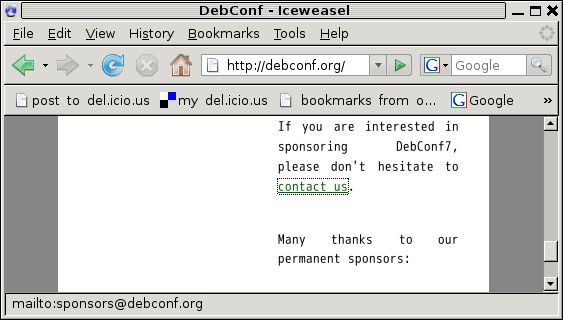
\includegraphics[width=1\hsize]{image200707/debconf-sponsor.png}
\end{center}
\caption{Debconf.org のウェブページ}
\end{figure}

 \url{http://www.debconf.org}にアクセスすると、コンタクト先がかいてありま
す。このメールアドレスに、スポンサーしたい旨メールで表明してください。

%%% trivia quiz
\dancersection{Debian Weekly News trivia quiz}{上川 純一}

ところで、Debian Weekly News (DWN)は読んでいますか?
Debian 界隈でおきていることについて書いているDebian Weekly News.
毎回読んでいるといろいろと分かって来ますが、一人で読んでいても、解説が少
ないので、
意味がわからないところもあるかも知れません。みんなでDWNを読んでみましょう。

漫然と読むだけではおもしろくないので、DWNの記事から出題した以下の質問にこたえてみてください。
後で内容は解説します。

\subsection{2007年6号}
\url{http://www.debian.org/News/weekly/2007/06/}
にある7月3日版です。

\santaku
{Andr\'e Luiz Rodrigues Ferreira が宣言したのはどのウェブサイトか}
{Debian art}
{Debian pop}
{Debian tart}
{A}

\santaku
{J\"ulich で行われた会議で lenny のリリースプロセスについて何をすることが決まったか}
{秘密のプロセスにのっとり、今後リリースがどうなっているかは非公開にする}
{毎月か二ヶ月に一回の最終週にリリース状況についてのメールを出す}
{安全保障のため今後は Debian Developerでないとリリースの状況がわからないようにする}
{B}

\santaku
{Lucas Nussbaum は毎月何をすると発表したか}
{深刻な問題のあるパッケージを順番にのっとる}
{深刻な問題のあるパッケージを管理している人に罰ゲームをさせる}
{深刻な問題のあるパッケージについて通知するメールを自動で送付}
{C}

\santaku
{Alexander Wirt は何を発表したか}
{backports.org が sid に対応}
{backports.org が lenny に対応}
{backports.org が etch に対応}
{C}

\santaku
{Martin Michlmyr が挑戦しているのは何か}
{Debian を gcc 4.2でビルドできるようにする}
{Debian を全部 C++ におきかえる}
{Debian を全部 ruby におきかえる}
{A}

\dancersection{最近のDebian関連のミーティング報告}{上川 純一}

\subsection{東京エリアDebian勉強会28回目報告}
% (query-replace-regexp "<.*?>" "")
% (query-replace-regexp "^[ 	]*" "")

東京エリアDebian勉強会参加報告。
5月の第28回東京エリアDebian勉強会を実施しました。

今回の参加者は
前田さん、やまねさん、出井さん、kinnekoさん、
hamanoさん、小室さん、鈴木さん、武藤さん、
山下さん、あけどさん、岩松さん、
noriaki satoさん、山本浩之さん、
山辺義孝さん、本庄さん、キタハラさん、
鈴木邦男さん、えとーさん、荒木さん、David Smith さん、
Charles Plessy さん、後藤さん、上川の23 人でした。

最近のイベントの紹介として、最初に前回の報告を行いました。
前回は主要な分散バージョン管理ツールについての特集でした。

DWNクイズを今回も実施しました。
全員に起立してもらい、グー・チョキ・パーで選択してもらいました。
1問目は一人しか正解しませんでした。
alioth にて、 git は昔からサポートされていており、今回サポートが追加されたのはMercurialです。
しかたないので、2問目からしきりなおし、最後まで4人ほどのこりました。
勝者には上川からここには書けないような豪華景品を贈呈しました。おめでとうございます。


次に、Debian Conferenceに向けて実施している準備の紹介を行いました。
pbuilder と superh についてのプレゼンテーションを行うことになっているの
ですが、リハーサルとして、Debian勉強会にて今回内容を説明しました。

最初にpbuilder について上川が紹介しました。
Debian ソースパッケージを処理してバイナリをつくる際に、
クリーンルーム環境を利用する、その手順をまとめたツールです、ということを紹介しました。


次に岩松さんが Debian の superh の移植版の紹介をしていました。
過去の歴史について力をいれて紹介していました。

kinneko さんがSH2A版のポートをやっている人もいるので紹介するのがよいだろうという指摘をしました。

上川の感想ですが、Debconfで紹介する目的として、新しい開発
者を募集するのが目的なのであれば、歴史については簡単にまと
めてしまって、SuperHの開発に使える機種の情報や何が面白いの
か、現状のポートのステータス、連絡先やレポジトリやウェブサ
イトの情報、どういう課題があるのかに力をいれて紹介するのが
よいのではないかという印象をうけました。

小室さんがその後に「サーバをエッチにしてみました」という題
でネタを披露しました。いろいろとトラブルがありそれを解決し
ました、ということだったのですが、「エッチにアップグレード
するのは簡単だということがわかりました」というので話をしめ
たので一同爆笑しました。


いつもとタイミングを変えてみて、その後に事前課題の紹介を行
いました。内容は「エッチになって困った事」にしてみました。
みんないろいろと思うところがあるようで議論が沸騰しました。
webminがなくなったこと、xlock がないこと、xorg になってし
まい設定が大きく変わっていること、udev の使いかたがよくわ
からないこと、カーネルがアップグレードするのでカーネル関連
の問題(ACPIなど)にぶつかる可能性があること、などが話題に
でました。/var/lock/apache2/ の権限が www-data ではなく 
root になってしまっているので webdav で書き込めないことな
どが紹介されていました(\debianbug{420101})。
apt-setup が削除されているのも仕様ですね。CUIで sources.list を編集するツールがあるのか?という話題が出ましたが、 vi をつかえ、と。

エッチにアップグレードする際に、どうやってみんなは情報をえ
ていて、どういうふうに情報を提供しているのだろう、という話
をしました。リリースノートを読むだとか、バグレポートを探す
だとか、MLに投稿するだとか、建前はおいておいて、現実のフロー
がどうなっているのかを語ってみました。どうやら、問題があれ
ばIRCでまず質問してみて、google で検索してみて、いろいろと
ためした結果を blog に書いている、というのが現実的なようで
す。そして、2ch などで同様の質問がされたら、 blogで書かれ
ている内容をまとめなおしてスレッドテンプレにまとめなおされ
るという流れになっているようです。言語が英語である点などか
らBTSは敷居の高く感じている人が多いようで、また複合的な問
題はパッケージ単位でしか登録できないBTSにはそぐわないため、
そういう情報の流れになっているようです。現実を見据えて今後
どうしていくべきか、悩ましいところです。

今回は宴会は
時の居酒屋  刻 荻窪店
にて開催しました。
料理がおいしかったです。

\subsection{東京エリアDebian勉強会29回目報告}
% (query-replace-regexp "<.*?>" "")
% (query-replace-regexp "^[ 	]*" "")

6月の第29回東京エリアDebian勉強会を英国スコットランド エジンバラにて実施
しました。

今回のDebian勉強会は、Debconf 向けの特別開催です。irc.debian.or.jp の 
\#debconf7 (文字コード: iso-2022-jp) にて現地の中継をかねて開催していま
す。今回何を実現するのか、それぞれ宣言をしてみました。

\begin{itemize}
 \item 岩松さんは superh のプレゼンの準備をしています。
 \item 矢吹さんは小林さんのプレゼンをかわりに実施するために準備をするようです。
 \item 上川は qemubuilder を実用にするためのいろいろな技をこなします。
\end{itemize}

\subsection{FSIJ 月例会 2007年7月}

Debian Conference 2007 の報告を産業総合研究所秋葉原サイトにて開催された
2007年7月開催の SEA \& FSIJ 合同フォーラムにて報告しました。岩松 信洋と
上川 純一が参加し、Debconf7での議題等について議論しました。 各種議題で議
論したのですが、SuperH のDebian 移植版について特に活発な討論が行われ、今
後の普及に向けての整備課題があきらかになってきました。今後の SuperH アー
キテクチャの活躍に期待です。

\dancersection{Debconf 参加報告}{岩松 信洋}
\label{sec:debconfreportsummary}
\index{Debconf2007}
\index{Debconf}

\subsection{Debconfとは}

  2007年度の Debconf は 6月13日から6月23日まで、英国スコットランドのエジ
ンバラで行われました。日本からは、上川 純一、矢吹 幸治、岩松 信洋が参加
しました。

\subsubsection{Debconfの歴史・経緯}

Debian Conference \url{http://debconf7.debconf.org/} は Debian 
の開発者たちが一同に介するイベントです。通常顔をあわせることのないメンバー
たちが一同に介し友好を深め、技術的な議論を戦わせます。過去の開催履歴を見
てみると\tbref{tab:debconflist}のようになります。

\begin{table}[H]
\caption{歴代のDebconf参加者推移}
\label{tab:debconflist}
 \begin{center}
 {\footnotesize
 \begin{tabular}{|c|c|c|r|}
 \hline
 年 & 名前 & 場所 & 参加人数 \\
 \hline
 2000 & debconf 0 &フランス ボルドー & \\
 2001 & debconf 1 &フランス ボルドー & \\
 2002 & debconf 2 &カナダ トロント & 90名 \\
 2003 & debconf 3 &ノルウェー オスロ & 140名 \\
 2004 & debconf 4 &ブラジル ポルトアレグレ &  150名 \\
 2005 & debconf 5 &フィンランド ヘルシンキ & 200名 \\
 2006 & debconf 6 &メキシコ オアスタペック & 300名 \\
 2007 & debconf 7 &英国スコットランド エジンバラ & 約400名 \\
 \hline
 \end{tabular}
 }
 \end{center}
\end{table}

\subsubsection{Debconf 2007}

2007年度のDebconfの会場はエジンバラ大学の学生会館 Teviot を活用しました。
専用のネットワーク回線をはりめぐらせ、無線LANネットワークもはりめぐらせ
ました。

また、Teviot は 夜10時に閉鎖する必要があったので、夜の会場(night venue) 
というものも準備されました、現在売り物件となっている使われていない教会を
使用し、ハックラボにしました。パイプオルガンなどがあり、風情がありました。
パイプオルガンはもともと壊れていたのですが、Debconf の会期中に修復され、
演奏会が催されました。

宿泊は会場から徒歩5分程度に位置する Budget Backpackers と Cowgate hostel 
という二つのホステルに分散して行いました。

\subsection{スコットランド/エジンバラ}

\subsubsection{行き方}
  日本からエジンバラまでは、直行便がありません。パリ経由か、ロンドン経由等で一回
  トランジットが必要です。距離は約10000km。飛行時間は約14時間かかります。
  上川、岩松組はパリの シャルル・ド・ゴール国際空港経由、矢吹はヒースロー経由で入国しました。

\subsubsection{会場}

\begin{wrapfigure}{r}{11cm}
  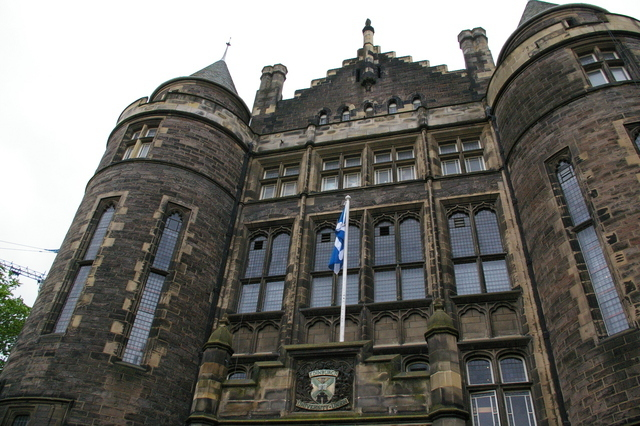
\includegraphics[width=5cm]{image200706/teviot.jpg}
  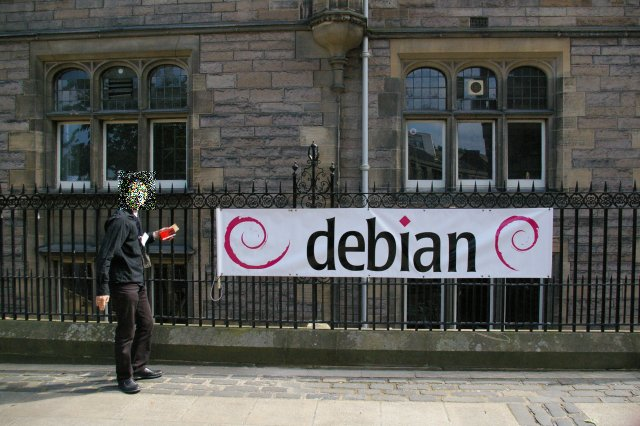
\includegraphics[width=5cm]{image200706/debconf7-debian.jpg}
\end{wrapfigure}
  会場は、エジンバラ大学の建物の一部である Teviot という名前の
  建物を借り切り、開催されました。

 参加者はふたつのホテルに分散して宿泊していたのですが、それらのホテルから歩いて
  10 分ほどのところにあります。
\\

\begin{itemize}
  \item Upper Talk Room: 	メイン用。250人ほど入ることができます。\\
	\begin{minipage}{0.4\hsize}
	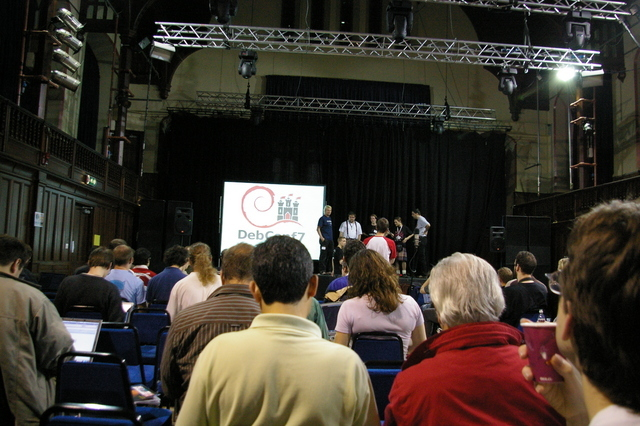
\includegraphics[width=0.8\hsize]{image200706/debconf7-upper-talk.jpg}
	\end{minipage}
  \item Basement Talk Room\\
	サブ用。50人ほど入ることができます。
  \item Lower BoF Room\\
	BOF 用。20人ほど入ることができます。
  \item Upper BoF Room\\
	BOF 用。20人ほど入ることができます。
  \item Hacklab 1: 	ハック用。\\
	\begin{minipage}{0.4\hsize}
	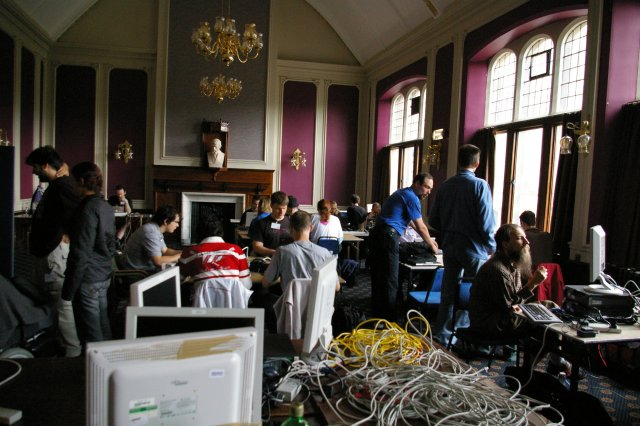
\includegraphics[width=0.8\hsize]{image200706/debconf7-hacklab00.jpg}
	\end{minipage}

  \item Hacklab 2: ハック用。通常はバーらしいです。\\
	\begin{minipage}{0.4\hsize}
	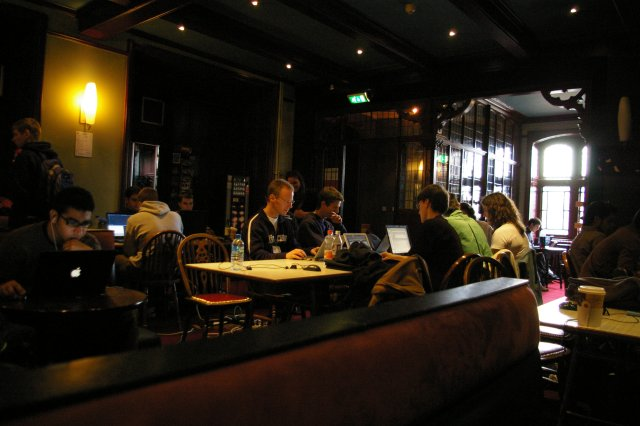
\includegraphics[width=0.8\hsize]{image200706/debconf7-hacklab01.jpg}
	\end{minipage}
  \item Night venue:
	廃墟と化した教会。パイプオルガンがあったりします。
	夜の22時以降は Teviot を使うことができないので
	ここを借りてみんなでハックしたり、話し合ったりしました。
\\
     	\begin{minipage}{0.4\hsize}
     	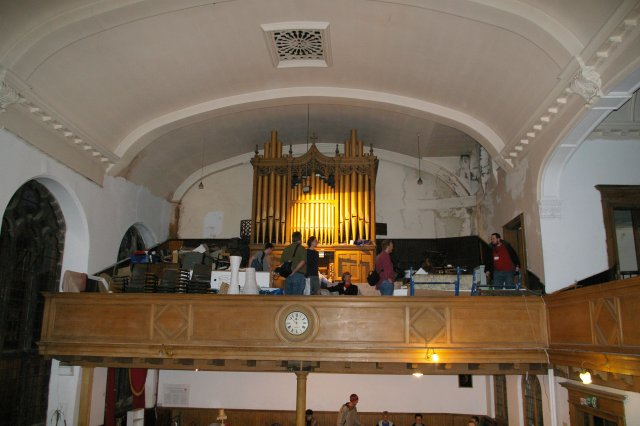
\includegraphics[width=0.8\hsize]{image200706/debconf7-elsewhere.jpg}
     	\end{minipage}
     	\begin{minipage}{0.4\hsize}
     	\end{minipage}
\end{itemize} 

\subsection{スケジュール}

\begin{wrapfigure}{r}{8cm}
 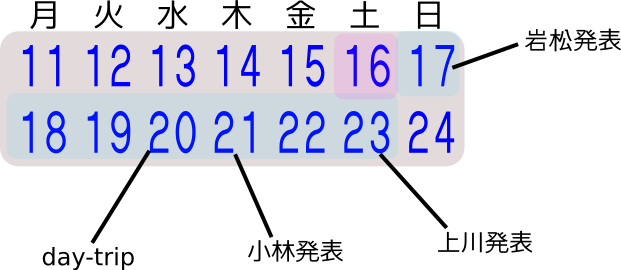
\includegraphics[width=1\hsize]{image200707/schedule.png}
\caption{全体スケジュール}
\label{fig:schedule}
\end{wrapfigure}
16日のDebian Day で Debian Conference は開始し、23日まで毎日いろいろな予
定がくまれていました。
20日だけはカンファレンス参加者で day-trip を実施しました。

\begin{wrapfigure}{r}{8cm}
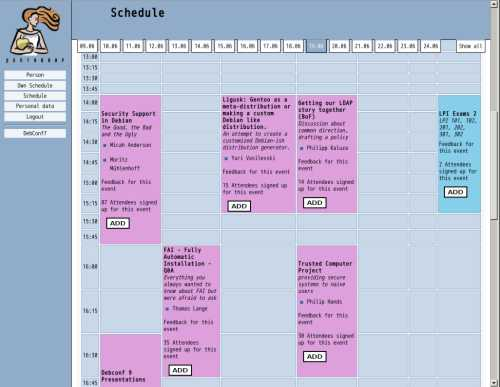
\includegraphics[width=8cm]{image200707/penta.png}
\caption{pentabarf 画面}
\label{fig:penta}
\end{wrapfigure}
 スケジュールは ruby-on-rails で実装された 
pentabarf システム(\fgref{fig:penta})で管理していました。
スケジュールには
随時変更がかかり、IRC bot での通知がなかったら誰も状況においつけなかっ
 たでしょう。


\subsection{主となった討論}

\subsubsection{組込み系についての白熱した議論}

ARM EABI の導入が大きなトピックです。日本から SuperH の
話題ももっていきました。マインドシェアがおおきくなっているようです。
また、組込関係の対応を Debian で行うための議論も行われました。
New DPL の Sam Hocevar が組込み関係に興味があるようなので、
いままで停滞していた組込み関係による成果のマージが加速するかもしれません。

\subsubsection{バージョン管理システムとソースコード管理の話}

git の利用方法のチュートリアルや、arch を例にとってのDebianディストリビュー
ションのフォークをメンテナンスするためのソースコード管理のやりかたについ
ての紹介がありました。git などの普及により分散SCMが普及し、ソースコード
の管理のワークフローに影響しており、再考が必要だという風潮が見られました。

特に ubuntu でソースコード管理を見直しており、bazaarを中心としてブランチ
をdpatchのパッチファイルに変換したりするツールなどのインフラがととのい始
めているということが大きいようです。

\subsubsection{翻訳についての議論}

翻訳関係の話が毎日行われました。毎日議論を重ね、議論した結果を毎晩ドキュメント
を修正していました。
また、時期リリースの lenny までに、翻訳のインフラやドキュメント整理
を行う予定だそうです。

小林さんの翻訳関係のインフラに関するセッションがあったのですが、
小林さんが来られなかったので、上川さんが代理で BOF を行いました。
各国で使用されているツールの紹介などがありました。日本でも導入を検討
をする必要がありそうです。

\subsubsection{Daytrip}


\begin{wrapfigure}{r}{5cm}
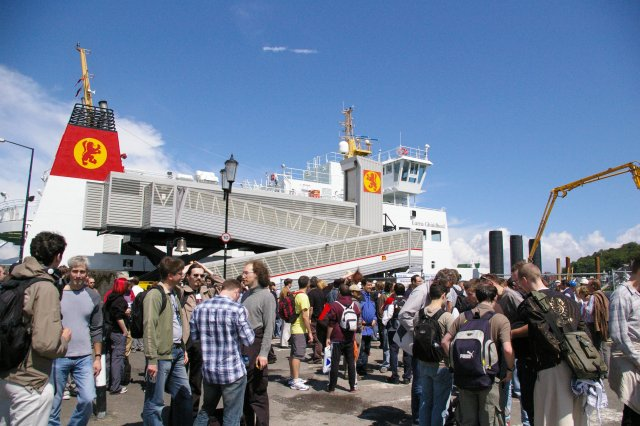
\includegraphics[width=5cm]{image200706/debconf7-daytrip.jpg}
\end{wrapfigure}

Debconf では一日、参加者で旅行をするというイベントがあります。今回の
Debconfでは Rotheway (Bute島) でまったりとピクニックをしました。Rotheway 
への移動は、Edinburgh から Glasgow へ電車で移動し、Glasgow からさらに電
車で Wemyss Bay へ移動します。Wemyss Bay は Rotheway 行き専用の舟着き場
で、そこから船に乗って Rotheway に移動しました。

Rotheway の町は島で、特になにもないところです。ほとんどの建物は売出中で、
裁判所の建物も売りに出ていました。財政がやばそうな感じです。
建造物としては、教会や、バイキングの侵略の際に戦った城がありましたが、修復中でしかも工事は止まっていました。
山の奥へ1時間ほど歩くと、湖があり、大抵の参加者はその湖でピクニックをしたり、ボード
に乗って遊んでいたようです。

\dancersection{将来の Debconf }{上川 純一}
\label{sec:debconfplanning}
\index{Debconf}


Debconf は来年はアルゼンチンですが、将来的には日本でも開催できるとよいで
すね。
また、Debconfの開催内容をいかに有益に使えるか、考えてみましょう。


\subsection{成果の活用}

Debian Conferenceには複数の側面があります。成果はどうやってできるのでしょ
うか。

\begin{table}[H]
\caption{参加の成果}
\label{tab:framework}
\begin{center}
{\LARGE
  \begin{tabularx}{\hsize}{|c|X|X|}
 \hline
 & 参加した場合 & 参加しなかった場合 \\
 \hline
 コード	& 合宿してコードがかける &  \\
 \hline
 文書化	& 合宿して文書がかける&  \\
 \hline
 議論 	& 直接議論できる &  \\
 \hline
 発表 	& セッションに参加して発表でき、発表をきくことができる。 &  \\
 \hline
&&\\
 \hline
&&\\
 \hline
 \end{tabularx}
}
\end{center} 
\end{table}

これを踏まえると、開催自体は重要ですが、参加にはおよびません。
あなたも参加したくなってきたのではないですか?

\subsection{日本開催}

Debian Developer の中では Debian Conference を日本で開催したいと思ってい
るメンバーがいます。日本で開催するとすれば、日本で開催するためのチームが
必要です。日本で数度イベントを運営して円滑にすすめられるようにしておくこ
とも必要でしょう。

日本でのDebconfの検討の進捗については
\url{http://wiki.debian.org/DebConfInJapan}
で整理されています。

\begin{table}[H]
\caption{2005年に実施した各種空港に到着するまでのコスト評価例}
\label{tab:framework}
\begin{center}
{\LARGE
  \begin{tabularx}{\hsize}{|c|X|X|X|}
 \hline
 & フランス & アメリカ & 南米 \\
 \hline
成田 & 828 & 809 & 1600 \\
千歳 &980 & 1197 &2121 \\
関西 &736 & 809 &1718 \\
沖縄 &1485 & 1197 &4307 \\
 \hline
 \end{tabularx}
}
\end{center} 
\end{table}

\dancersection{今後の予定}{上川 純一}

\subsection{次回}
次回は8月18日に東京エリアDebian勉強会があります。cdn.debian.or.jp につい
ての紹介と apt の sources.list の設定方法について紹介する予定です。

\subsection{OSC Tokyo/Fall}

10月5日・6日に開催されます。Debian JP も参加するのであれば準備を検討する
必要があります。

\cleartooddpage

\begin{minipage}[b]{0.2\hsize}
 \colorbox{dancerlightblue}{\rotatebox{90}{\fontsize{80}{80} {\gt デビアン勉強会} }}
\end{minipage}
\begin{minipage}[b]{0.8\hsize}

\vspace*{15cm}
{\color{dancerlightblue}\rule{\hsize}{1mm}}
\vspace{2mm}

\includegraphics[width=2cm]{image200502/openlogo-nd.eps}
\noindent \Large \bf Debian 勉強会資料\\ \\
\noindent \normalfont \debmtgyear{}年\debmtgmonth{}月\debmtgdate{}日 \hspace{5mm}  初版第1刷発行\\
\noindent \normalfont 東京エリア Debian 勉強会 (編集・印刷・発行)\\
{\color{dancerdarkblue}\rule{\hsize}{1mm}}
\end{minipage}

\end{document}
